\chapter{Solução Proposta}

Esse capitulo discorre sobre a solução que está sendo proposta, como o sistema foi pensado, suas características, o processo que o usuário irá seguir, para se ter uma visão geral do que é o sistema e qual é o objetivo do sistema e para quem ele está sendo feito. 

O seu diferencial, que será, por meio de indicadores, auxiliar os gestores nas suas tomadas de decisão quanto ao setor de manutenção e os técnicos, quanto a estratégia de manutenção que será escolhida para cada tipo de equipamento. O sistema foi pensado como um módulo do software já existente e utilizado, o SIPAT.

%------------------------------------------------------------------------------------------------------------------------%

\section{Visão Geral do Sistema}

\textbf{Oportunidade de Negócios}

O setor de manutenção vem ganhando grande espaço nas organizações e empresas, por poder ser um grande diferencial na qualidade dos serviços internos oferecidos, para o ambiente de trabalho e de grande economia nos gastos. 

Tendo em vista essa preocupação crescente em como melhorar a qualidade e aumentar o ciclo de vida dos ativos (equipamentos, bens e outros), esse sistema é proposto, para que a UnB, possa ter um gerenciamento eficaz da manutenção e que traga resultados contudentes e que possam ser anasildados e incorparados as decisões gerenciais da instituição. Assim como, ter os objetivos do setor alinhados aos objetivos da universidade.

\textbf{Descrição do Problema}

\begin{table}[H]
\centering
\caption{Descrição do Problema. Fonte: Autor.}
\label{tab-problema}
\begin{tabular}{ | p{5cm} | p{10cm} | }
\hline
	\textbf{O problema} & Falta de um sistema que controle o gerenciamento da manutenção de forma eficaz e completa.  \\ \hline
	\textbf{afeta} & Processo de manutenção, disponibilidade, confiabilidade dos equipamentos e gastos realizados com o setor de manutenção. \\ \hline
	\textbf{O seu impacto é} & Conseguir ter maior controle sobre os gastos e a qualidade dos equipamentos da universidade. \\ \hline
	\textbf{Uma solução ideal seria} & Um sistema que contemplasse todas as características observadas no setor de manutenção e que mostre relatórios que auxiliem nas tomadas de decisões gerenciais. \\ \hline
\end{tabular}
\end{table}

\pagebreak

\textbf{Sentença de Posição do Produto}

\begin{table}[H]
\centering
\caption{Sentença de Posição do Produto. Fonte: Autor.}
\label{tab-produto}
\begin{tabular}{ | p{5cm} | p{10cm} | }
\hline
	\textbf{Para} & Setor de Manutenção. \\ \hline
	\textbf{Quem} & Ténicos e Gestores. \\ \hline
	\textbf{O Sistema de Gerenciamento da Manutenção} & É um software. \\ \hline
	\textbf{Que} & Acompanha o ciclo de manutenção de equipamentos e auxilia nas tomadas de decisões. \\ \hline
	\textbf{Diferente de} & O sistema atual que apenas permite acompanhar as ordens de serviços abertas. \\ \hline
	\textbf{Nosso produto} & Sistema que acompanha o ciclo de manutenção de equipamentos e auxilia nas tomadas de decisões. \\ \hline
\end{tabular}
\end{table}

\textbf{Demografia do Mercado}

O mercado-alvo desse sistema compreende instituições e empresas com grande e diversificado número de ativos, que suportam atividades chaves e precisam ter alta disponibilidade e confiabiliade.

\textbf{Ambiente do Usuário}

O usuário do sistema irá ustilizá-lo no mesmo ambiente do SIPAT, pois ele foi pensado para ser um módulo do mesmo. Portanto, será instalado nos computadores da universidade, o usuário deverá solicitar sua instalação ao CPD, e ele será utilizado pela intranet da instituição.

\textbf{Resumo dos Usuários}

\begin{table}[H]
\centering
\caption{Resumo dos Usuários do Sistema. Fonte: Autor.}
\label{tab-resumo-usuarios}
\begin{tabular}{ | p{2cm} | p{7cm} | p{5cm} | }
\hline
	\textbf{Nome} & \textbf{Descrição} & \textbf{Papel} \\ \hline
	\textbf{Técnico} & Usuário que irá monitorar as manutenções pelo sistema. Incluir no sistemas os dados das manutenções realizadas, que alimentarão os relatórios que o sistema disponibiliza. & Abrir ordens de serviços. Incluir informações das manutenções realizadas. \\ \hline
	\textbf{Gestor} & Usuário que irá acompanhar o andamento da manutenções, por meio das informações do sistema, relatórios e gráficos. & Imprimir relatórios, visualizar gráfico. \\ \hline
\end{tabular}
\end{table}

\pagebreak

\textbf{Perfil dos Usuários}

\begin{table}[H]
\centering
\caption{Perfil do Técnico. Fonte: Autor.}
\label{tab-perfil-tec}
\begin{tabular}{ | p{5cm} | p{10cm} | }
\hline
	\textbf{Descrição} & Pessoa que irá alimentar o sistema com os dados de manutenção dos equipamentos. Irá abrir ordens de serviços e após a manutenção ser realizada, irá fechá-la.  \\ \hline
	\textbf{Tipo} & Usuário experiente. \\ \hline
	\textbf{Responsabilidades} &  Revisar os requisitos e os designs da Interface de Usuário. Fornecer feedback regular após a release do produto. \\ \hline
	\textbf{Critérios de Sucesso} & Precisa ser capaz de importar os equipamentos, visualizá-los, escolher o tipo de manutenção dos equipamentos, abrir e fechar ordens de serviços, inserir informações das manutenções realizadas, visulizar gráficos de acompanhamento do estado dos equipamentos, visualizar relatórios. \\ \hline
	\textbf{Envolvimento} & Revisor de requisitos. \\ \hline
	\textbf{Produtos Liberados} & Relatórios de uso/visualização. \\ \hline
	\textbf{Comentários/Problemas} & Nenhum. \\ \hline
\end{tabular}
\end{table}

\begin{table}[H]
\centering
\caption{Perfil do Gestor. Fonte: Autor.}
\label{tab-perfil-gestor}
\begin{tabular}{ | p{5cm} | p{10cm} | }
\hline
	\textbf{Descrição} & Pessoa que irá visualizar os relatórios, gráficos e consultar as informações sobre as manutenções e equipamentos. \\ \hline
	\textbf{Tipo} & Usuário primário. \\ \hline
	\textbf{Responsabilidades} & Consumidor básico das informações do sistema. \\ \hline
	\textbf{Critérios de Sucesso} & gráficos e consultar as informações sobre as manutenções e equipamentos. \\ \hline
	\textbf{Envolvimento} & Utilização do sistema. \\ \hline
	\textbf{Produtos Liberados} & Consultas e relatórios. \\ \hline
	\textbf{Comentários/Problemas} & Nenhum. \\ \hline
\end{tabular}
\end{table}

\pagebreak

\textbf{Necessidades dos Usuários}


\begin{table}[H]
\centering
\caption{Problemas que devem ser resolvidos pelo Sistema de Manutenção de Equipamentos. Fonte: Autor.}
\label{tab-necessidade}
\begin{tabular}{ | p{3cm} | p{2cm} | p{3cm} | p{3cm} | p{4cm} |}
\hline
	\textbf{Necessidade} & \textbf{Prioridade} & \textbf{Preocupações} & \textbf{Solução Atual} & \textbf{Soluções Propostas} \\ \hline
	Importar dados dos equipamentos & Alta & Volume de dados & Acoplado ao sistema de patrimônio & Importar os dados para o sistema de manutenção \\ \hline
	Agrupar equipamentos por especificação e grupo & Média & Nenhuma & Equipamentos são classificados por especificação e grupo & Conseguir visualizar os equipamentos por especificação e grupo \\ \hline
	Visualizar quantidade de equipamentos parados, em uso e em manutenção & Alta & Transformar informações em gráfico & Não existe & Mostrar em uma listagem pelas classificações e geral em um gráfico \\ \hline
	Visualizar relatórios (gastos totais, ordens de serviços e indicadores de eficiência) & Alta & Qualificar os dados dos indicadores de eficiência & Não existe & Disponibilizar os relatórios. \\ \hline
	Escolher tipo de manutenção & Alta & Nenhuma & Seção de manutenção preventiva & Disponibilizar opção de escolher o tipo de manutenção por equipamento \\ \hline
	Abrir ordem de serviço & Média & Nenhuma & Já existe no SIPAT & Possibilitar abrir uma nova ordem de serviço pelo sistema  \\ \hline
	Visualizar ordens de serviços abertas para um equipamento & Média & Nenhuma & Já existe no SIPAT & Possibilitar visualização de uma listagem das ordens de serviço \\ \hline
	Adicionar  componentes de um equipamento que devem ser trocados nas manutenções preventivas & Alta & Nenhuma & Não existe & Possibilitar adição dos componentes principais de um equipamento \\ \hline
	Visualizar dados cadastrais de um equipamento & Baixa & Nenhuma & Já existe no SIPAT & Possibilitar a visualização dos dados cadastrais pelo sistema de manutenção \\ \hline
	Visualizar indicadores do equipamento & Alta & Nenhuma & Não existe & Possibilitar visualização de indicadores \\ \hline
\end{tabular}
\end{table}
 
%--------------------------------------------------------------------------------------------%

\section{Requisitos do Sistema}

Os requisitos do sistema foram elicitados a partir das referências bibliográficas, resultado de pesquisas feitas sobre quais são as características que um CMMS deve ter (Tabela~\ref{comparativo}), qual o processo que esse tipo de ferramenta deve seguir, da reunião realizada com os técnicos do CPD e esntrevistas realizadas com o técnico da DIMEQ, para descobrir o que eles precisam de um sistema de manutenção, o que eles sentem falta que poderia ajudar a menlhorar a rotina e gerar resultados melhores.

Assim como, a partir da visão do sistema na Tabela~\ref{tab-necessidade}, onde foram resumidas as necessidades e características para a modelagem do sistema. 

Por ser um sistema novo para Universidade, para ajudar e facilitar o entendimento do que seria necessário, para tornar visível o que era pedido, foi, antes de elicitados os requisitos, prototipadas as telas do sistema e modelado o fluxo que seria seguido (seção~\ref{to-be}. Os protótipos encontram-se no APÊNDICE B.

Abaixo estão listados os requisitos elicitados para o sistema:

\begin{enumerate}
	\item Técnico e Gestor visualizam, na página principal, um gráfico com a quantidade de equipamentos \textit{em uso, em manutenção e parados}.
	\item Técnico e Gestor visualizam, na página principal, uma listagem com os equipamentos classificados por grupo e especificação.
	\item Técnico e Gestor visualizam relatórios disponibilizados pelo sistema.
	\item Técnico importa equipamentos do SIPAT para o sistema.
	\item Técnico e Gestor visualizam listagem de uma especificação com todos os seus equipamentos.
	\item Técnico e Gestor visualizam gráfico com quantidade de equipamentos \textit{em uso, em manutenção e parados}, de uma certa especificação e grupo.
	\item Técnico escolhe o tipo de manutenção que será realizada em um equipamento.
	\item Técnico adiciona os componentes principais de um equipamento.
	\item Técnico visualiza os dados cadastrais do equipamento.
	\item Tecnico abre ordem de serviço.
	\item Técnico visualiza ordens de serviços abertas pelo SIPAT.
	\item Técnico  e Gestor visualizam indicadores dos equipamentos.
	\item Técnico visualiza listagem com manutenções a serem feitas.
	\item Técnico e Gestor escolhem tipo de relatório que querem visualizar.
\end{enumerate}

%-----------------------------------------------------------------%

\subsection{Diagrama de Caso de Uso}

Para descrever as funcionalidades do sistema, foram utilizados casos de uso, que são uma forma de representar uma funcionalidade de um software em formato de texto, detalhando e especificando o que tal funcionalidade irá fazer. Para ter uma visão de como essas funcionalidades interagem com o usuário, foi desenhado o diagrama de caso de uso mostrado na Figura~\ref{diagrama-de-caso-de-uso}. 

\graphicspath{{figuras/}}
\begin{figure}[H]
\centering
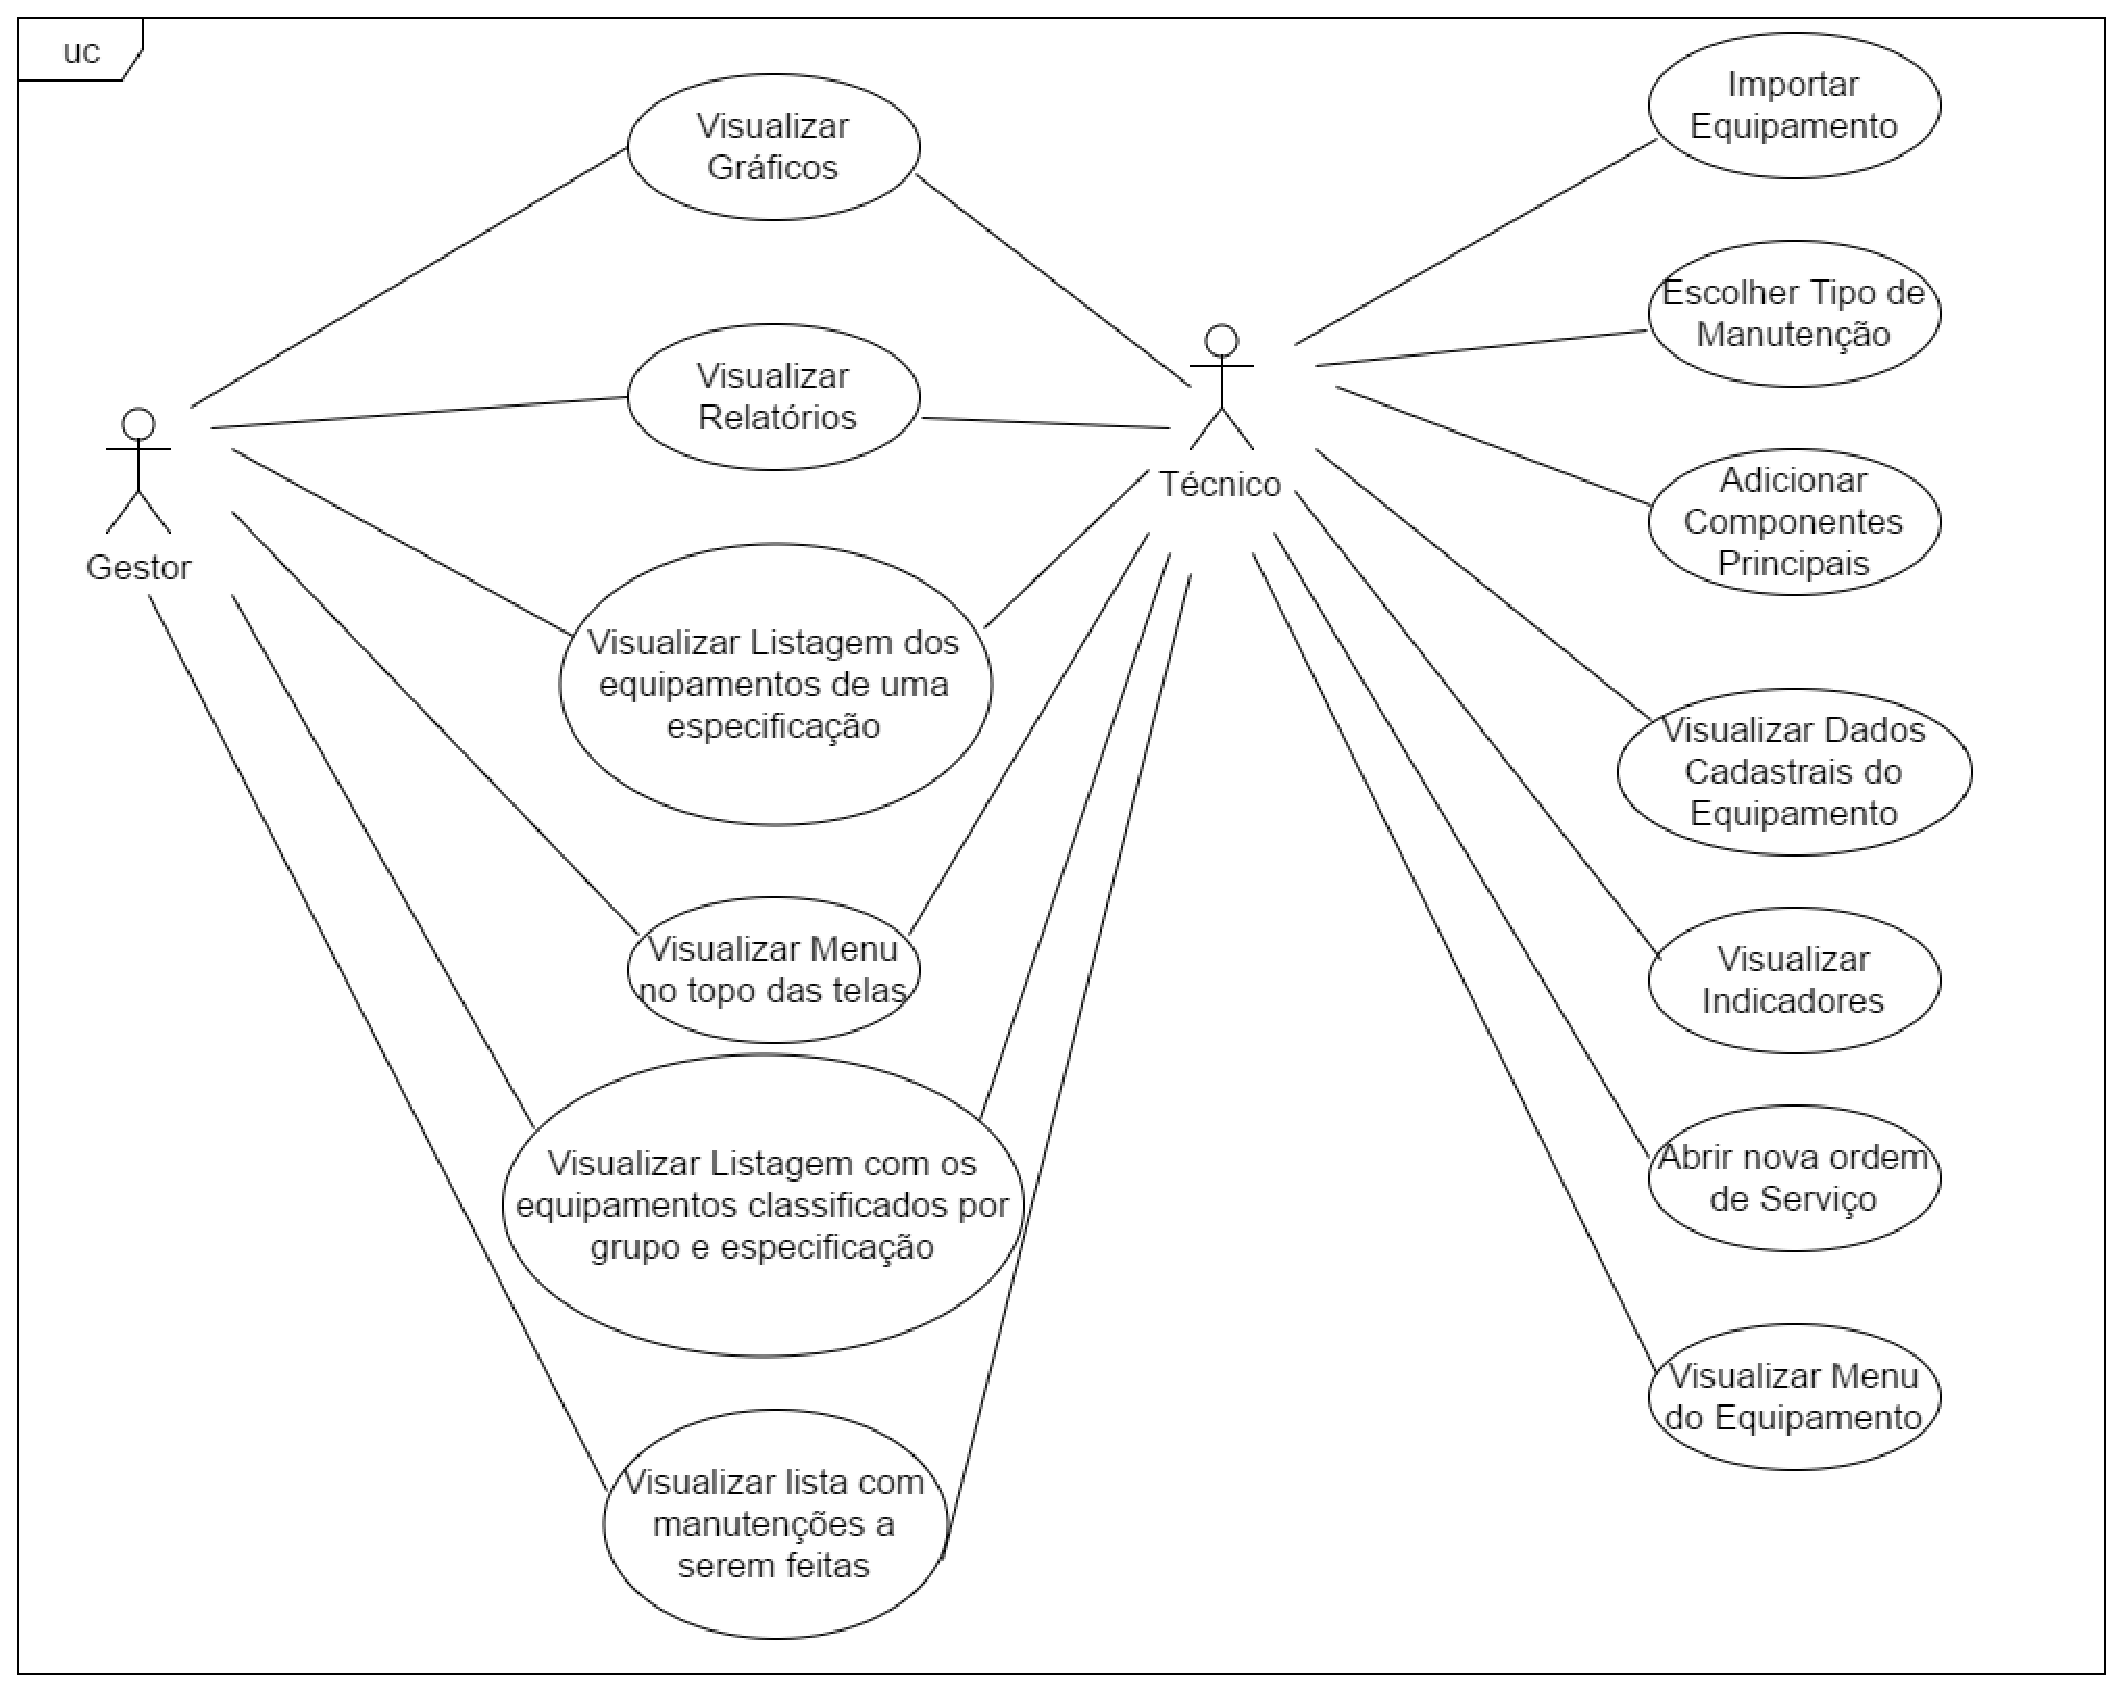
\includegraphics[width=1.0\textwidth]{diagrama-de-caso-de-uso}
\caption{Diagrama de Caso de Uso do Sistema. \textbf{Fonte: Autor.}}
\label{diagrama-de-caso-de-uso}
\end{figure}

Os Casos de Uso mostrados no diagrama acima, foram todos especificados, e se encontram no APÊNDICE A do trabalho.

%-----------------------------------------------------------------%

\subsection{Modelo de Domínio}

O Modelo de Domínio é utilizado para representar classes conceituais ou objetos do mundo real em um domínio, ou seja, mostra de forma visual qual o problema a ser resiolvido pelo sistema. Para isso, é necessário identificar os conceitos relacionados aos requisitos, analisar o problema que o sistema buscar resolver de forma conceitual.

Ele não pertence ao domínio da solução, como o diagrama de classe, e portanto não deve ser utilizado para modelar a arquitetura so software, seu papel é representar o problema por meio de um diagrama. Não deve ser associado

Sua modelagem é feita utilizando os elementos da notação UML para diagrama de classes. É composto basicamente por:

\begin{itemize}
	\item Conceitos (classes conceituais);
	\item Atributos;
	\item Relacionamento entre classes conceituais.
\end{itemize}


%---------------------------------------------------------------------------------------------------------------%

\section{Processo TO BE}
\label{to-be}

O processo TO BE é a sugestão de melhorias e remodelamento do processo AS IS, explicado na Seção~\ref{processo-as-is}. Esse fluxo foi modelado, a partir dos protótipos e da observação e estudo das regras de negócio presentes no processo AS IS, o qual foi feito junto ao técnico da DIMEQ. 

A sequência das atividades foi baseada no fluxo montado com as telas prototipadas, seguindo o caminho, a partir da importação dos dados dos equipamentos, seguindo para as configurações individuais dos equipamentos, análise dos indicadores, escolha do tipo de manutenção, e decisão, tendo como base as informações mostradas no sistema (relatórios, indicadores, etc) se o equipamento será mantido, substituído, se mudará o tipo de manutenção, entre outros.

O fluxo principal (Figura~\ref{processo-to-be}), possui um subrocesso, mostrado na Figura~\ref{subprocesso-to-be}, para realização de visita técnica, o qual foi extraído do processo AS IS, e não foi modificado. Isso porque, a forma com que as visitas para a avaliação e reparo dos equipamentos, extrapola o escopo da proposta do trabalho, que tem por objetivo, acompanhar o ciclo de vida do equipamento por meio do sistema aqui modelado. 


\begin{landscape}
\graphicspath{{figuras/}}
\begin{figure}[H]
\centering
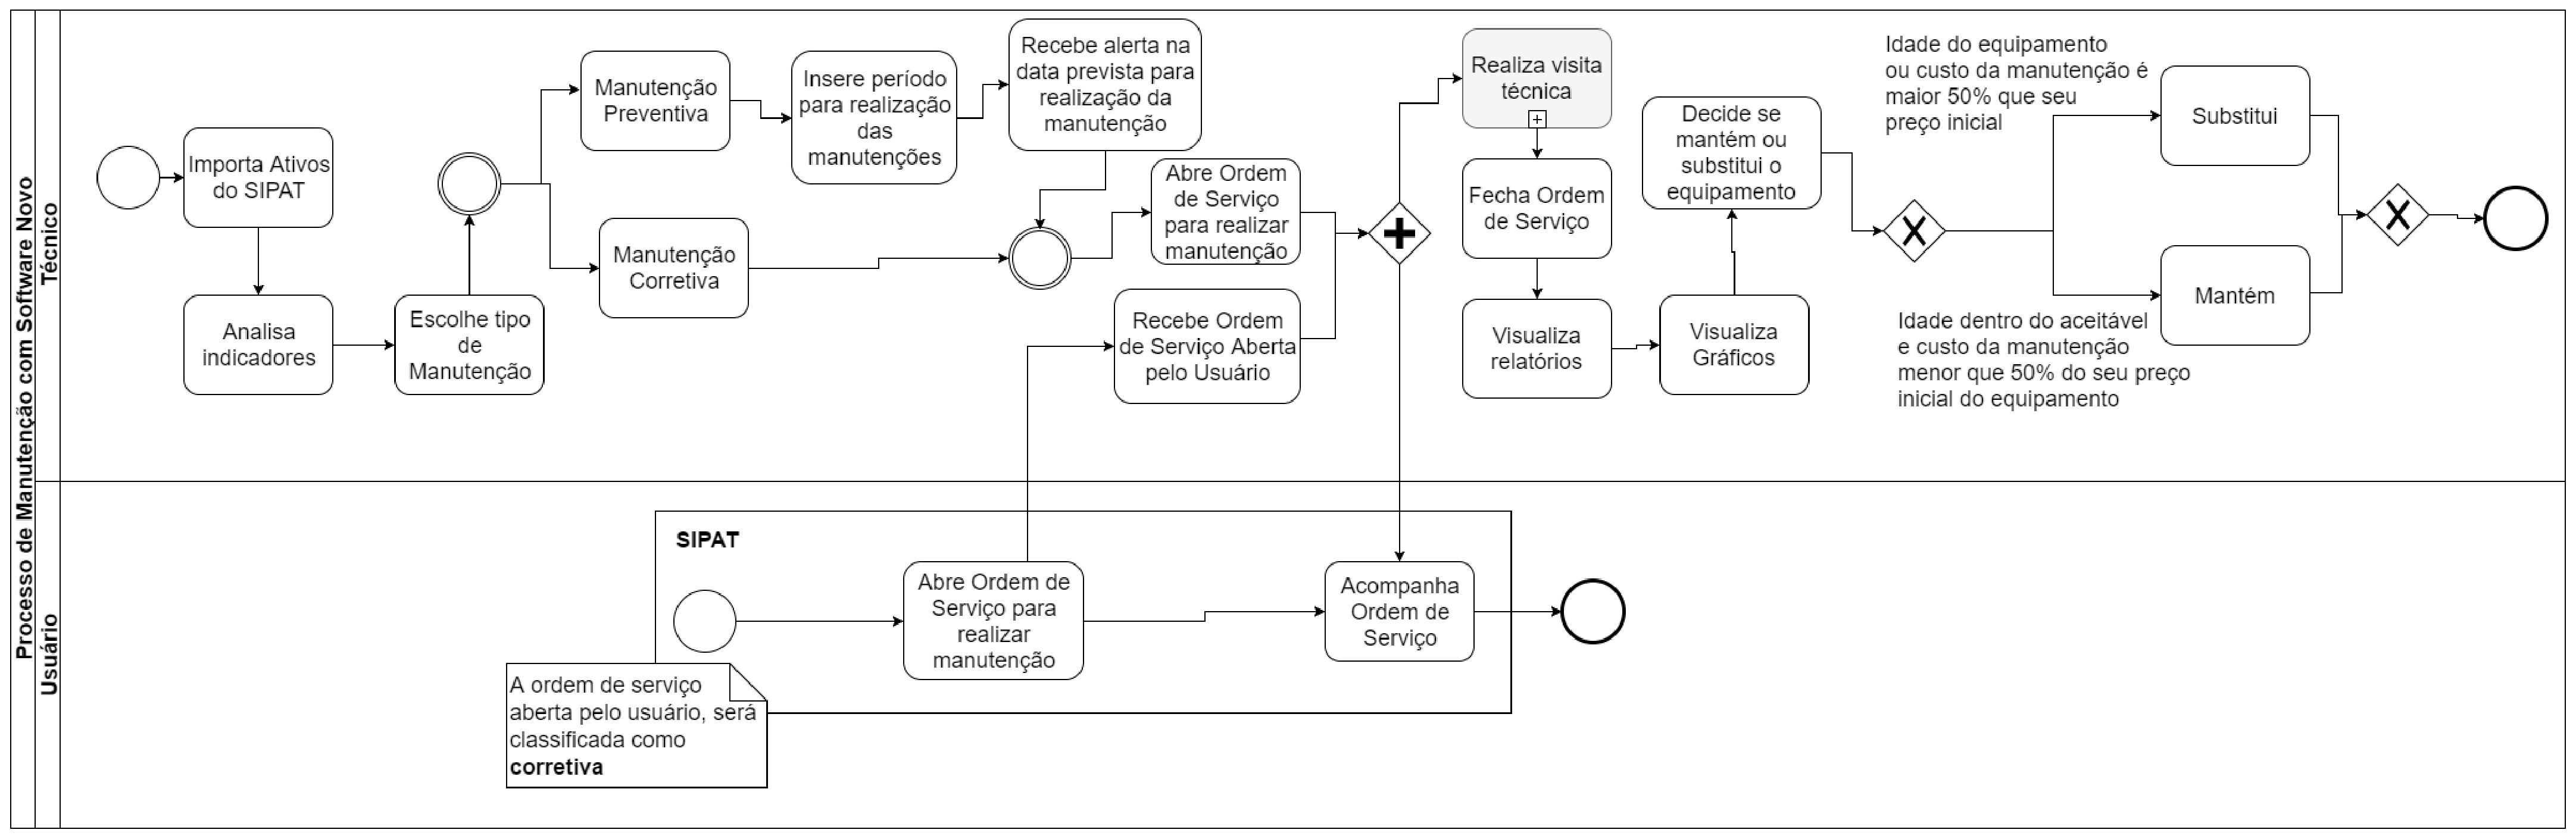
\includegraphics[width=1.5\textwidth]{processo_to_be}
\caption{Processo TO BE. \textbf{Fonte: Autor.}}
\label{processo-to-be}
\end{figure}
\end{landscape} 


\begin{landscape}
\graphicspath{{figuras/}}
\begin{figure}[H]
\centering
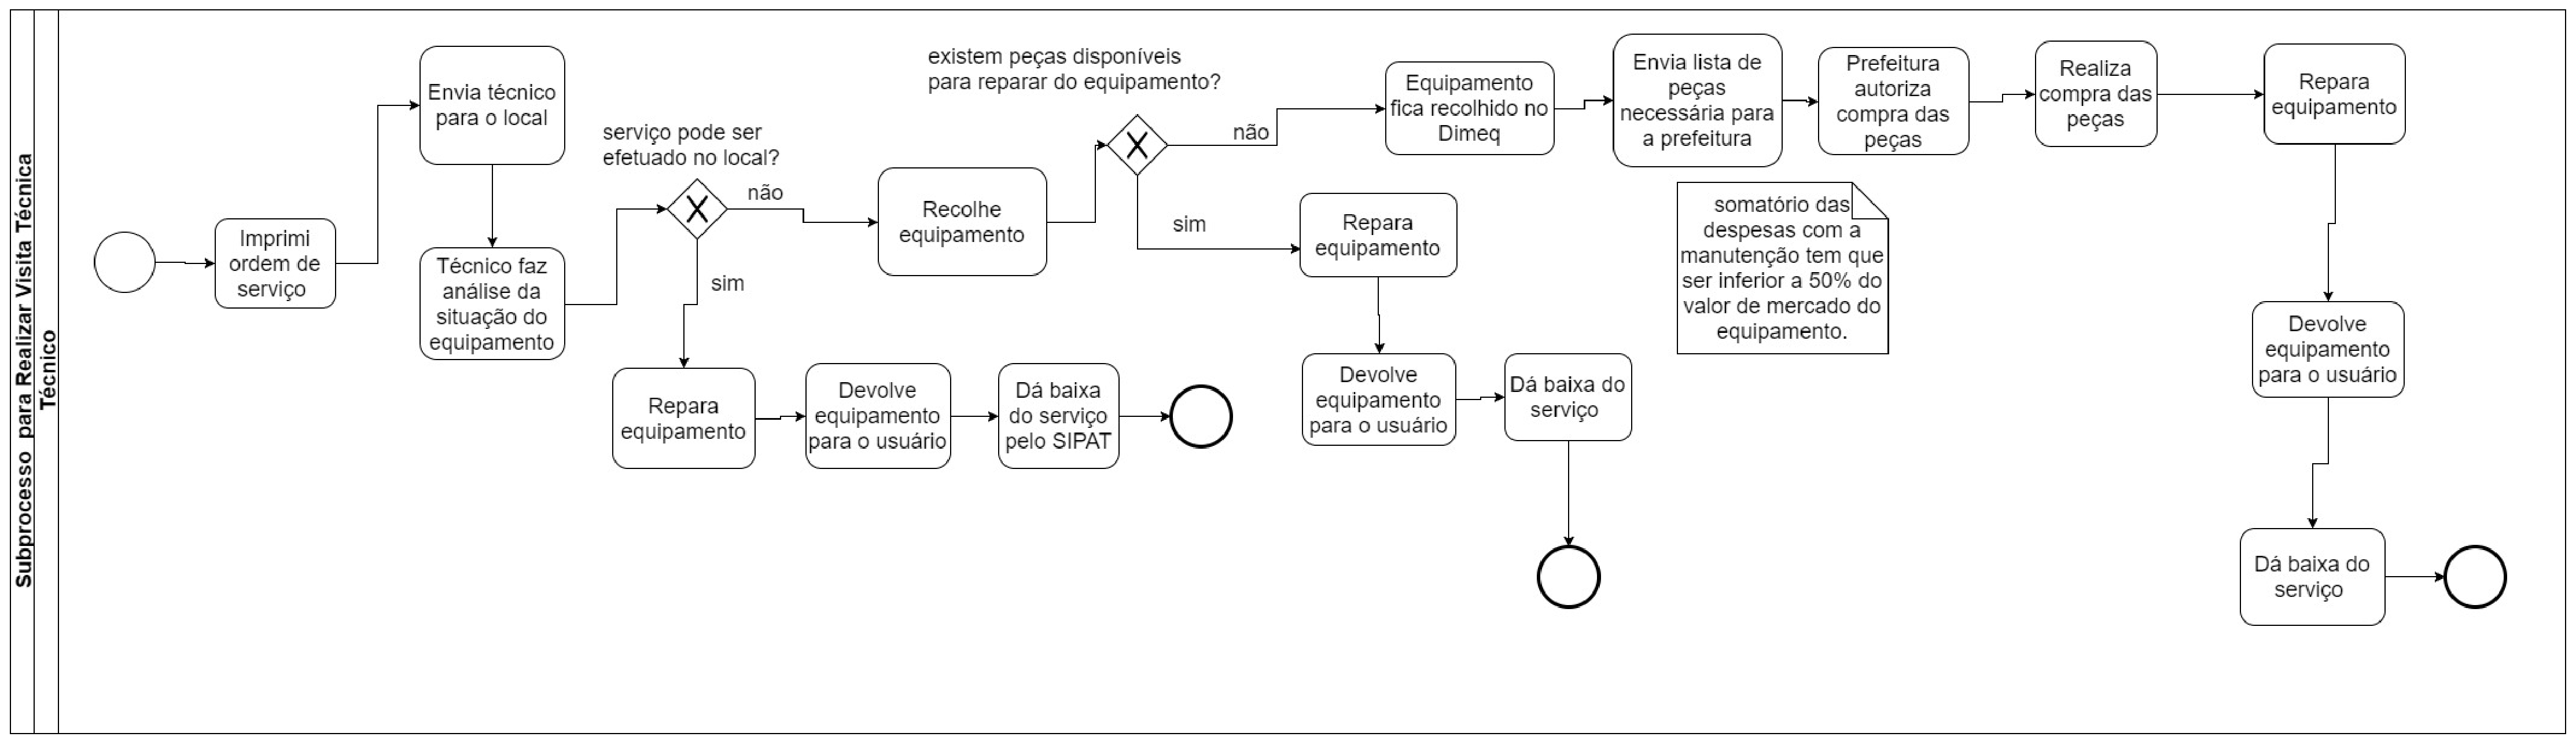
\includegraphics[width=1.5\textwidth]{subprocesso_to_be}
\caption{Processo para realizar visita técnica. \textbf{Fonte: Autor.}}
\label{subprocesso-to-be}
\end{figure}
\end{landscape} 

%---------------------------------------------------------------------------------------------------------------%

